% This is samplepaper.tex, a sample chapter demonstrating the
% LLNCS macro package for Springer Computer Science proceedings;
% Version 2.21 of 2022/01/12
%
\documentclass[runningheads]{llncs}
%

%
\usepackage[T1]{fontenc}
\usepackage{comment}
% T1 fonts will be used to generate the final print and online PDFs,
% so please use T1 fonts in your manuscript whenever possible.
% Other font encondings may result in incorrect characters.
%
\usepackage{graphicx}
% Used for displaying a sample figure. If possible, figure files should
% be included in EPS format.
%
% If you use the hyperref package, please uncomment the following two lines
% to display URLs in blue roman font according to Springer's eBook style:
%\usepackage{color}
%\renewcommand\UrlFont{\color{blue}\rmfamily}
%\urlstyle{rm}
%
\begin{document}
%\bibliographystyle{splncs04}
%\bibliography{LLMs and Data Streams}
%
\title{Large Language Models and Data Streams}
%
%\titlerunning{Abbreviated paper title}
% If the paper title is too long for the running head, you can set
% an abbreviated paper title here
%
\author{Silyu Li}
%
%\authorrunning{F. Author et al.}
% First names are abbreviated in the running head.
% If there are more than two authors, 'et al.' is used.
%
\institute{RWTH Aachen University, Aachen, Germany
%\email{lncs@springer.com}\\
%\url{http://www.springer.com/gp/computer-science/lncs} \and
%ABC Institute, Rupert-Karls-University Heidelberg, Heidelberg, Germany\\
%\email{\{abc,lncs\}@uni-heidelberg.de}
}
%
\maketitle              % typeset the header of the contribution
%
\begin{abstract}
    Large language models, such as ChatGPT, have become widely recognized and are extensively utilized across various domains. However, these models are typically trained on static datasets, lacking updates to new data beyond their initial training set. To enable models that can continuously update themselves based on incoming data, it is necessary to have large language models trained and updated on input data streams.

    In this paper, we begin by outlining the structure and fundamental applications of large language models. Subsequently, we introduce the concept of data streams and provide an overview of current use cases where large language models are adapted to accommodate streaming data. Finally, we summarize the existing challenges associated with integrating large language models with data streams and discuss potential solutions.
\keywords{LLM  \and data streams \and chatGPT.}
\end{abstract}
%
%
%
\section{Introduction}
In this part I would like to mainly talk about the motivation of this seminar paper, which is about the fact that large language models are trained based on certain static datasets that will not automatically be updated, and this causes the resulted models to only be able to access information from its training datasets. But in many scenarios such models can't satisfy our needs, for example if we want to have traffic prediction based on real time traffic data,
monitor news and events sentiment to help predict finacial market, monitor health condition based on real-time health data and etc.
So In order to have models that can fulfill those use cases, we need to find and compare useful methods that combine large language models and continuous data input (data streams) together, and also summarize the current major obstacles. 

\section{Related Works}
In this chapter I will talk about the concepts and techniques that are related to this topic

\subsection{Large Language Model}
In this subsection I will talk about following aspects of large language models:
    \subsubsection{The component of large language models}
      \begin{itemize}
        \item Transformer architecture: neural network architectures designed to handle sequential data, such as text, effectively
        \item Self-attention mechanism: enables the model to capture dependencies between words in a sentence more effectively.
        \item Embedding layer:  converts words or tokens into high-dimensional vectors, which represent their semantic meaning in the context of the sentence.
        \item Encoder layers: help the model to encode the input text into a meaningful representation.
        \item Decoder layers: consist of self-attention mechanisms and feed-forward neural networks, but they also include additional attention mechanisms to focus on relevant parts of the input during the decoding process.
        \item Positional encoding: added to the input embeddings to provide information about the position of each word in the sequence.
        \item Output layer: takes the final representation produced by the decoder layers and maps it to the output vocabulary.
        \item Softmax: convert the raw scores into probabilities.
      \end{itemize}
    \subsubsection{The evolution of large language models}
      \begin{itemize}
        \item Earliest simple models: relied on statistical methods and shallow learning techniques.
        \item Models using deep learning techniques: recurrent neural networks (RNNs) and long short-term memory (LSTM) 
        \item Models using tranformer architecture: revolutionized natural language processing (NLP) by allowing models to capture dependencies between words more effectively through attention mechanisms.
        \item Models using BERT technique: further improved language understanding by pre-training models on large corpora of text in both forward and backward directions. 
        \item GPT series: trained on massive datasets.
        \item Future trend: continual increase in model size and training data.
      \end{itemize}
    \subsubsection{The use case of large language models} 
    
    It has huge potential and capabilities such as language translation, text classification,
    content generation, chatbots etc.


\subsection{Data Stream}
In this subsection I will talk about following aspects of data streams:
%\begin{itemize}
    \subsubsection{The definition of data streams} With the definition from different sources
    \subsubsection{The use case of data streams} Large amount of real-time data is very useful in many application fields such as Weather Forecasting, Health monitoring, Internet of Things etc.
%\end{itemize}

\section{Use Cases and Obstacles}
In this section I will give an overview of current use cases where large language models and data streams are combined together, and also summarize the major obstacles of combining large language models with data streams. Furthermore I will also give an introduction of what measurements have been taken to mitigate the obstacles. 
\subsection{Use Cases}
Following use cases will be covered:
\begin{itemize}
    \item Social Media Monitoring: Analyzing streaming data from social media platforms can help monitor regional news, sentiment, and trends in real-time.
    \item Financial Monitoring:  Large language models can analyze streaming news feeds to identify important events, trends, and sentiment in real-time. This can be valuable for financial institutions, and risk management companies to stay informed about current events and market trends.
    \item Health Care Monitoring: Large language models can analyze streaming medical data such as patient records, diagnostic reports, and research papers to assist healthcare providers in diagnosing diseases, identifying treatment options, and monitoring public health trends in real-time.
    \item Traffic Data Monitoring: Large language models can analyze streaming traffic data to monitor traffic conditions in real-time to help reduce traffic accidents and level up transportation efficiency. 
    %\item Security and Threats Detection: Large language models can analyze streaming data from network logs, security alerts, and threat intelligence feeds to detect and respond to cybersecurity threats in real-time. This includes identifying suspicious activities, malware signatures, and potential vulnerabilities.
\end{itemize}

\subsection{Obstacles and Methods}
Following obstacles will be covered:
\begin{itemize}
    \item Concept Drift: if the LLM is trained for a long time, it is possible that the relationship between the inputs and the outputs itself might change.
    \item Computational Resources: continuous learning requires significant computational resources, which may be costly or impractical to scale.
    \item Privacy and Security:  streaming data often contains sensitive or private information, raising concerns about data privacy and security.
    \item Data Quality: data streams may contain noisy or unreliable information, leading to incorrect model updates.
\end{itemize}
\noindent
Following measurements will be covered:
\begin{itemize}
    \item Using data preprocessing techniques to filter out noise and ensure data quality. Use anomaly detection algorithms to identify and remove outliers in the data. Employ quality assurance measures to verify the accuracy of incoming data.
    \item Continuously monitor model performance and detect concept drift using statistical methods or machine learning algorithms. Implement adaptive learning techniques to update the model in response to concept drift. Periodically retrain the model on recent data batches to maintain accuracy.
    \item Optimize model architectures and algorithms to reduce computational overhead. Utilize distributed computing frameworks to parallelize model training and inference tasks.
    \item Implement data anonymization and encryption techniques to protect sensitive information during data transmission and storage
\end{itemize}
%\paragraph{Following measurements will be covered:}

\section{Conclusion}
In this section I will shortly summarize the outline of this paper and also talk about the possible future development of large language models using data streams.

%\paragraph{Sample Heading (Fourth Level)}
%The contribution should contain no more than four levels of
%headings. Table~\ref{tab1} gives a summary of all heading levels.
\begin{comment}
\begin{table}
\caption{Table captions should be placed above the
tables.}\label{tab1}
\begin{tabular}{|l|l|l|}
\hline
Heading level &  Example & Font size and style\\
\hline
Title (centered) &  {\Large\bfseries Lecture Notes} & 14 point, bold\\
1st-level heading &  {\large\bfseries 1 Introduction} & 12 point, bold\\
2nd-level heading & {\bfseries 2.1 Printing Area} & 10 point, bold\\
3rd-level heading & {\bfseries Run-in Heading in Bold.} Text follows & 10 point, bold\\
4th-level heading & {\itshape Lowest Level Heading.} Text follows & 10 point, italic\\
\hline
\end{tabular}
\end{table}


\noindent Displayed equations are centered and set on a separate
line.
\begin{equation}
x + y = z
\end{equation}
Please try to avoid rasterized images for line-art diagrams and
schemas. Whenever possible, use vector graphics instead (see
Fig.~\ref{fig1}).

\begin{figure}
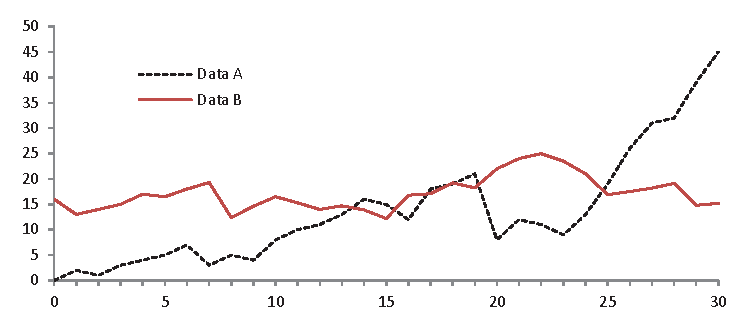
\includegraphics[width=\textwidth]{fig1.eps}
\caption{A figure caption is always placed below the illustration.
Please note that short captions are centered, while long ones are
justified by the macro package automatically.} \label{fig1}
\end{figure}

\begin{theorem}
This is a sample theorem. The run-in heading is set in bold, while
the following text appears in italics. Definitions, lemmas,
propositions, and corollaries are styled the same way.
\end{theorem}
%
% the environments 'definition', 'lemma', 'proposition', 'corollary',
% 'remark', and 'example' are defined in the LLNCS documentclass as well.
%
\begin{proof}
Proofs, examples, and remarks have the initial word in italics,
while the following text appears in normal font.
\end{proof}
For citations of references, we prefer the use of square brackets
and consecutive numbers. Citations using labels or the author/year
convention are also acceptable. The following bibliography provides
a sample reference list with entries for journal
articles~\cite{ref_article1}, an LNCS chapter~\cite{ref_lncs1}, a
book~\cite{ref_book1}, proceedings without editors~\cite{ref_proc1},
and a homepage~\cite{ref_url1}. Multiple citations are grouped
\cite{ref_article1,ref_lncs1,ref_book1},
\cite{ref_article1,ref_book1,ref_proc1,ref_url1}.

\begin{credits}
\subsubsection{\ackname} A bold run-in heading in small font size at the end of the paper is
used for general acknowledgments, for example: This study was funded
by X (grant number Y).

\subsubsection{\discintname}
It is now necessary to declare any competing interests or to specifically
state that the authors have no competing interests. Please place the
statement with a bold run-in heading in small font size beneath the
(optional) acknowledgments\footnote{If EquinOCS, our proceedings submission
system, is used, then the disclaimer can be provided directly in the system.},
for example: The authors have no competing interests to declare that are
relevant to the content of this article. Or: Author A has received research
grants from Company W. Author B has received a speaker honorarium from
Company X and owns stock in Company Y. Author C is a member of committee Z.
\end{credits}
\end{comment}
%
% ---- Bibliography ----
%
% BibTeX users should specify bibliography style 'splncs04'.
% References will then be sorted and formatted in the correct style.
%
\bibliographystyle{splncs04}
%\bibliography{LLMs and Data Streams}
%

\begin{thebibliography}{8}
\begin{comment}
\bibitem{ref_article1}
Author, F.: Article title. Journal \textbf{2}(5), 99--110 (2016)

\bibitem{ref_lncs1}
Author, F., Author, S.: Title of a proceedings paper. In: Editor,
F., Editor, S. (eds.) CONFERENCE 2016, LNCS, vol. 9999, pp. 1--13.
Springer, Heidelberg (2016). \doi{10.10007/1234567890             }

\bibitem{ref_book1}
Author, F., Author, S., Author, T.: Book title. 2nd edn. Publisher,
Location (1999)

\bibitem{ref_proc1}
Author, A.-B.: Contribution title. In: 9th International Proceedings
on Proceedings, pp. 1--2. Publisher, Location (2010)

\bibitem{ref_url1}
LNCS Homepage, \url{http://www.springer.com/lncs}, last accessed 2023/10/25
\end{comment}
\bibitem{Liu23}
Liu, Yiheng, Tianle Han, Siyuan Ma, Jiayue Zhang, Yuanyuan Yang, Jiaming Tian, Hao He et al. "Summary of chatgpt-related research and perspective towards the future of large language models." Meta-Radiology (2023): 100017.

\bibitem{Kasneci23}
Kasneci, Enkelejda, Kathrin Seßler, Stefan Küchemann, Maria Bannert, Daryna Dementieva, Frank Fischer, Urs Gasser et al. "ChatGPT for good? On opportunities and challenges of large language models for education." Learning and individual differences 103 (2023): 102274.

\bibitem{Thiru23}
Thirunavukarasu, Arun James, Darren Shu Jeng Ting, Kabilan Elangovan, Laura Gutierrez, Ting Fang Tan, and Daniel Shu Wei Ting. "Large language models in medicine." Nature medicine 29, no. 8 (2023): 1930-1940.

\bibitem{Chang23}
Chang, Yupeng, Xu Wang, Jindong Wang, Yuan Wu, Linyi Yang, Kaijie Zhu, Hao Chen et al. "A survey on evaluation of large language models." ACM Transactions on Intelligent Systems and Technology (2023).

\bibitem{Zhang23}
Zhang, Shuhao, Xianzhi Zeng, Yuhao Wu, and Zhonghao Yang. "Harnessing scalable transactional stream processing for managing large language models [vision]." arXiv preprint arXiv:2307.08225 (2023).

\bibitem{Zhang24}
Zhang, Kunpeng, Feng Zhou, Lan Wu, Na Xie, and Zhengbing He. "Semantic understanding and prompt engineering for large-scale traffic data imputation." Information Fusion 102 (2024): 102038.

\bibitem{Xu23}
Xu, Xuhai, Bingshen Yao, Yuanzhe Dong, Hong Yu, James Hendler, Anind K. Dey, and Dakuo Wang. "Leveraging large language models for mental health prediction via online text data." arXiv preprint arXiv:2307.14385 (2023).

\bibitem{Zhang_Xin24}
Zhang, Xin, Linhai Zhang, Deyu Zhou, and Guoqiang Xu. "Fine-grainedly Synthesize Streaming Data Based On Large Language Models With Graph Structure Understanding For Data Sparsity." arXiv preprint arXiv:2403.06139 (2024).

\bibitem{Wu24}
Wu, Tongtong, Linhao Luo, Yuan-Fang Li, Shirui Pan, Thuy-Trang Vu, and Gholamreza Haffari. "Continual learning for large language models: A survey." arXiv preprint arXiv:2402.01364 (2024).

\bibitem{Brown20}
Brown, Tom, Benjamin Mann, Nick Ryder, Melanie Subbiah, Jared D. Kaplan, Prafulla Dhariwal, Arvind Neelakantan et al. "Language models are few-shot learners." Advances in neural information processing systems 33 (2020): 1877-1901.

\bibitem{Gama13}
Gama, Joao, Raquel Sebastiao, and Pedro Pereira Rodrigues. "On evaluating stream learning algorithms." Machine learning 90 (2013): 317-346.

\bibitem{Jang21}
Jang, Joel, Seonghyeon Ye, Sohee Yang, Joongbo Shin, Janghoon Han, Gyeonghun Kim, Stanley Jungkyu Choi, and Minjoon Seo. "Towards continual knowledge learning of language models." arXiv preprint arXiv:2110.03215 (2021).

\bibitem{Geisler13}
Geisler, Sandra. "Data stream management systems." In Dagstuhl Follow-Ups, vol. 5. Schloss Dagstuhl-Leibniz-Zentrum fuer Informatik, 2013.

\bibitem{Geisler16}
Geisler, Sandra. "A systematic evaluation approach for data stream-based applications." PhD diss., Dissertation, RWTH Aachen University, 2016, 2016.

\bibitem{Vaswani17}
Vaswani, Ashish, Noam Shazeer, Niki Parmar, Jakob Uszkoreit, Llion Jones, Aidan N. Gomez, Łukasz Kaiser, and Illia Polosukhin. "Attention is all you need." Advances in neural information processing systems 30 (2017).

\bibitem{Devlin18}
Devlin, Jacob, Ming-Wei Chang, Kenton Lee, and Kristina Toutanova. "Bert: Pre-training of deep bidirectional transformers for language understanding." arXiv preprint arXiv:1810.04805 (2018).

\bibitem{Yenduri24}
Yenduri, Gokul, M. Ramalingam, G. Chemmalar Selvi, Y. Supriya, Gautam Srivastava, Praveen Kumar Reddy Maddikunta, G. Deepti Raj et al. "GPT (Generative Pre-trained Transformer)–A Comprehensive Review on Enabling Technologies, Potential Applications, Emerging Challenges, and Future Directions." IEEE Access (2024).

\bibitem{Lester21}
Lester, Brian, Rami Al-Rfou, and Noah Constant. "The power of scale for parameter-efficient prompt tuning." arXiv preprint arXiv:2104.08691 (2021).

\bibitem{So19}
So, David, Quoc Le, and Chen Liang. "The evolved transformer." In International conference on machine learning, pp. 5877-5886. PMLR, 2019.

\bibitem{Zhao22}
Zhao, Feng, Xinning Li, Yating Gao, Ying Li, Zhiquan Feng, and Caiming Zhang. "Multi-layer features ablation of BERT model and its application in stock trend prediction." Expert Systems with Applications 207 (2022): 117958.

\bibitem{Ren24}
Ren, Yilong, Yue Chen, Shuai Liu, Boyue Wang, Haiyang Yu, and Zhiyong Cui. "TPLLM: A Traffic Prediction Framework Based on Pretrained Large Language Models." arXiv preprint arXiv:2403.02221 (2024).

\bibitem{Liu24}
Liu, Chenxi, Sun Yang, Qianxiong Xu, Zhishuai Li, Cheng Long, Ziyue Li, and Rui Zhao. "Spatial-temporal large language model for traffic prediction." arXiv preprint arXiv:2401.10134 (2024).

\bibitem{Yang22}
Yang, Xi, Aokun Chen, Nima PourNejatian, Hoo Chang Shin, Kaleb E. Smith, Christopher Parisien, Colin Compas et al. "A large language model for electronic health records." NPJ digital medicine 5, no. 1 (2022): 194.

\bibitem{Gupta23}
Gupta, Kshitij, Benjamin Thérien, Adam Ibrahim, Mats L. Richter, Quentin Anthony, Eugene Belilovsky, Irina Rish, and Timothée Lesort. "Continual Pre-Training of Large Language Models: How to (re) warm your model?." arXiv preprint arXiv:2308.04014 (2023).

\bibitem{Naga23}
Naga Sanjay, "Continuous Training of ML models. A case-study on how to keep our machine learning models relevant.", Medium, June 25, 2023

\bibitem{Prapas21}
Prapas, Ioannis, Behrouz Derakhshan, Alireza Rezaei Mahdiraji, and Volker Markl. "Continuous training and deployment of deep learning models." Datenbank-Spektrum 21, no. 3 (2021): 203-212.

\end{thebibliography}

\end{document}
